% Standalone source of the figure fig:octree of the octree paper, written by make_fig_octree.py.
% Build: lualatex (or pdflatex) fig_octree.tex; the paper includes the PDF. Legible in grey scale.
\documentclass[border=3pt]{standalone}
\usepackage{amsmath,amssymb}
\usepackage{tikz}
\usetikzlibrary{arrows.meta,decorations.pathmorphing,calc}
\begin{document}
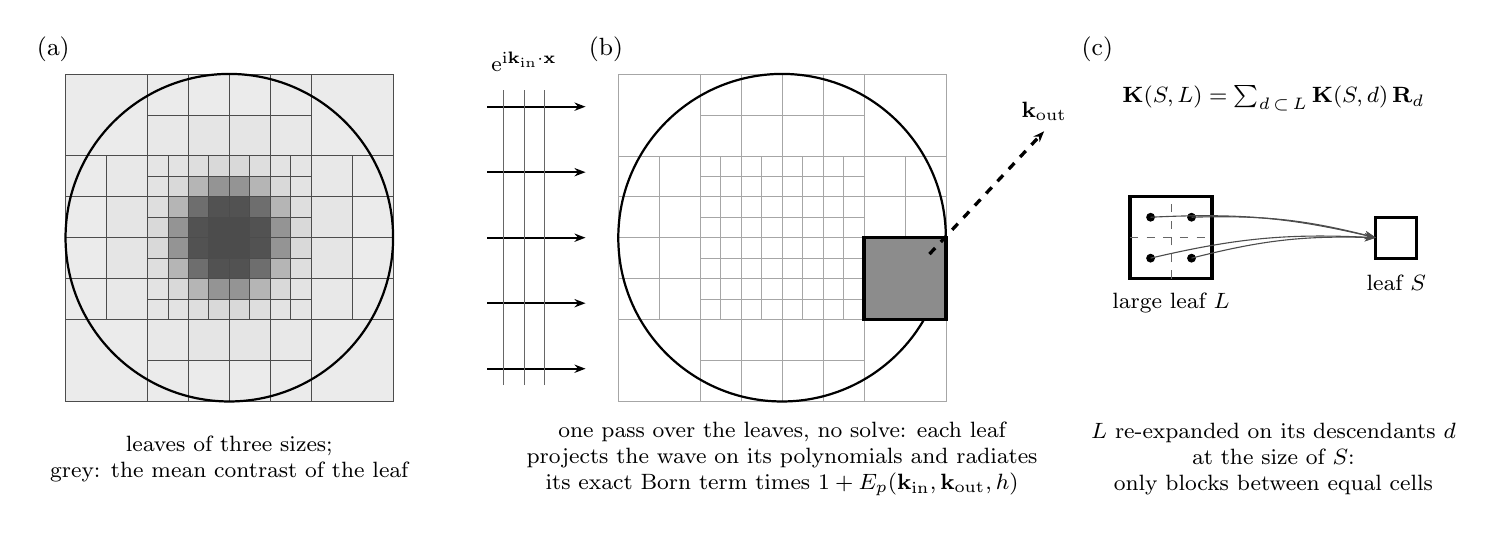
\begin{tikzpicture}[x=0.52cm, y=0.52cm, font=\small, >={Stealth[length=4pt]}]
  % ---------------------------------------------------------------- (a) the tree over the medium
  \begin{scope}
    \filldraw[fill=black!8, draw=black!70, line width=0.25pt] (2.000,2.000) rectangle ++(2.000,2.000);
    \filldraw[fill=black!8, draw=black!70, line width=0.25pt] (3.000,1.000) rectangle ++(1.000,1.000);
    \filldraw[fill=black!9, draw=black!70, line width=0.25pt] (2.000,1.000) rectangle ++(1.000,1.000);
    \filldraw[fill=black!8, draw=black!70, line width=0.25pt] (3.000,0.000) rectangle ++(1.000,1.000);
    \filldraw[fill=black!10, draw=black!70, line width=0.25pt] (2.000,0.000) rectangle ++(1.000,1.000);
    \filldraw[fill=black!8, draw=black!70, line width=0.25pt] (3.000,-1.000) rectangle ++(1.000,1.000);
    \filldraw[fill=black!10, draw=black!70, line width=0.25pt] (2.000,-1.000) rectangle ++(1.000,1.000);
    \filldraw[fill=black!8, draw=black!70, line width=0.25pt] (3.000,-2.000) rectangle ++(1.000,1.000);
    \filldraw[fill=black!9, draw=black!70, line width=0.25pt] (2.000,-2.000) rectangle ++(1.000,1.000);
    \filldraw[fill=black!8, draw=black!70, line width=0.25pt] (2.000,-4.000) rectangle ++(2.000,2.000);
    \filldraw[fill=black!8, draw=black!70, line width=0.25pt] (1.000,3.000) rectangle ++(1.000,1.000);
    \filldraw[fill=black!8, draw=black!70, line width=0.25pt] (0.000,3.000) rectangle ++(1.000,1.000);
    \filldraw[fill=black!9, draw=black!70, line width=0.25pt] (1.000,2.000) rectangle ++(1.000,1.000);
    \filldraw[fill=black!10, draw=black!70, line width=0.25pt] (0.000,2.000) rectangle ++(1.000,1.000);
    \filldraw[fill=black!10, draw=black!70, line width=0.25pt] (1.500,1.500) rectangle ++(0.500,0.500);
    \filldraw[fill=black!11, draw=black!70, line width=0.25pt] (1.000,1.500) rectangle ++(0.500,0.500);
    \filldraw[fill=black!11, draw=black!70, line width=0.25pt] (1.500,1.000) rectangle ++(0.500,0.500);
    \filldraw[fill=black!15, draw=black!70, line width=0.25pt] (1.000,1.000) rectangle ++(0.500,0.500);
    \filldraw[fill=black!13, draw=black!70, line width=0.25pt] (0.500,1.500) rectangle ++(0.500,0.500);
    \filldraw[fill=black!15, draw=black!70, line width=0.25pt] (0.000,1.500) rectangle ++(0.500,0.500);
    \filldraw[fill=black!29, draw=black!70, line width=0.25pt] (0.500,1.000) rectangle ++(0.500,0.500);
    \filldraw[fill=black!42, draw=black!70, line width=0.25pt] (0.000,1.000) rectangle ++(0.500,0.500);
    \filldraw[fill=black!13, draw=black!70, line width=0.25pt] (1.500,0.500) rectangle ++(0.500,0.500);
    \filldraw[fill=black!29, draw=black!70, line width=0.25pt] (1.000,0.500) rectangle ++(0.500,0.500);
    \filldraw[fill=black!15, draw=black!70, line width=0.25pt] (1.500,0.000) rectangle ++(0.500,0.500);
    \filldraw[fill=black!42, draw=black!70, line width=0.25pt] (1.000,0.000) rectangle ++(0.500,0.500);
    \filldraw[fill=black!57, draw=black!70, line width=0.25pt] (0.500,0.500) rectangle ++(0.500,0.500);
    \filldraw[fill=black!68, draw=black!70, line width=0.25pt] (0.000,0.500) rectangle ++(0.500,0.500);
    \filldraw[fill=black!68, draw=black!70, line width=0.25pt] (0.500,0.000) rectangle ++(0.500,0.500);
    \filldraw[fill=black!70, draw=black!70, line width=0.25pt] (0.000,0.000) rectangle ++(0.500,0.500);
    \filldraw[fill=black!15, draw=black!70, line width=0.25pt] (1.500,-0.500) rectangle ++(0.500,0.500);
    \filldraw[fill=black!42, draw=black!70, line width=0.25pt] (1.000,-0.500) rectangle ++(0.500,0.500);
    \filldraw[fill=black!13, draw=black!70, line width=0.25pt] (1.500,-1.000) rectangle ++(0.500,0.500);
    \filldraw[fill=black!29, draw=black!70, line width=0.25pt] (1.000,-1.000) rectangle ++(0.500,0.500);
    \filldraw[fill=black!68, draw=black!70, line width=0.25pt] (0.500,-0.500) rectangle ++(0.500,0.500);
    \filldraw[fill=black!70, draw=black!70, line width=0.25pt] (0.000,-0.500) rectangle ++(0.500,0.500);
    \filldraw[fill=black!57, draw=black!70, line width=0.25pt] (0.500,-1.000) rectangle ++(0.500,0.500);
    \filldraw[fill=black!68, draw=black!70, line width=0.25pt] (0.000,-1.000) rectangle ++(0.500,0.500);
    \filldraw[fill=black!11, draw=black!70, line width=0.25pt] (1.500,-1.500) rectangle ++(0.500,0.500);
    \filldraw[fill=black!15, draw=black!70, line width=0.25pt] (1.000,-1.500) rectangle ++(0.500,0.500);
    \filldraw[fill=black!10, draw=black!70, line width=0.25pt] (1.500,-2.000) rectangle ++(0.500,0.500);
    \filldraw[fill=black!11, draw=black!70, line width=0.25pt] (1.000,-2.000) rectangle ++(0.500,0.500);
    \filldraw[fill=black!29, draw=black!70, line width=0.25pt] (0.500,-1.500) rectangle ++(0.500,0.500);
    \filldraw[fill=black!42, draw=black!70, line width=0.25pt] (0.000,-1.500) rectangle ++(0.500,0.500);
    \filldraw[fill=black!13, draw=black!70, line width=0.25pt] (0.500,-2.000) rectangle ++(0.500,0.500);
    \filldraw[fill=black!15, draw=black!70, line width=0.25pt] (0.000,-2.000) rectangle ++(0.500,0.500);
    \filldraw[fill=black!9, draw=black!70, line width=0.25pt] (1.000,-3.000) rectangle ++(1.000,1.000);
    \filldraw[fill=black!10, draw=black!70, line width=0.25pt] (0.000,-3.000) rectangle ++(1.000,1.000);
    \filldraw[fill=black!8, draw=black!70, line width=0.25pt] (1.000,-4.000) rectangle ++(1.000,1.000);
    \filldraw[fill=black!8, draw=black!70, line width=0.25pt] (0.000,-4.000) rectangle ++(1.000,1.000);
    \filldraw[fill=black!8, draw=black!70, line width=0.25pt] (-1.000,3.000) rectangle ++(1.000,1.000);
    \filldraw[fill=black!8, draw=black!70, line width=0.25pt] (-2.000,3.000) rectangle ++(1.000,1.000);
    \filldraw[fill=black!10, draw=black!70, line width=0.25pt] (-1.000,2.000) rectangle ++(1.000,1.000);
    \filldraw[fill=black!9, draw=black!70, line width=0.25pt] (-2.000,2.000) rectangle ++(1.000,1.000);
    \filldraw[fill=black!15, draw=black!70, line width=0.25pt] (-0.500,1.500) rectangle ++(0.500,0.500);
    \filldraw[fill=black!13, draw=black!70, line width=0.25pt] (-1.000,1.500) rectangle ++(0.500,0.500);
    \filldraw[fill=black!42, draw=black!70, line width=0.25pt] (-0.500,1.000) rectangle ++(0.500,0.500);
    \filldraw[fill=black!29, draw=black!70, line width=0.25pt] (-1.000,1.000) rectangle ++(0.500,0.500);
    \filldraw[fill=black!11, draw=black!70, line width=0.25pt] (-1.500,1.500) rectangle ++(0.500,0.500);
    \filldraw[fill=black!10, draw=black!70, line width=0.25pt] (-2.000,1.500) rectangle ++(0.500,0.500);
    \filldraw[fill=black!15, draw=black!70, line width=0.25pt] (-1.500,1.000) rectangle ++(0.500,0.500);
    \filldraw[fill=black!11, draw=black!70, line width=0.25pt] (-2.000,1.000) rectangle ++(0.500,0.500);
    \filldraw[fill=black!68, draw=black!70, line width=0.25pt] (-0.500,0.500) rectangle ++(0.500,0.500);
    \filldraw[fill=black!57, draw=black!70, line width=0.25pt] (-1.000,0.500) rectangle ++(0.500,0.500);
    \filldraw[fill=black!70, draw=black!70, line width=0.25pt] (-0.500,0.000) rectangle ++(0.500,0.500);
    \filldraw[fill=black!68, draw=black!70, line width=0.25pt] (-1.000,0.000) rectangle ++(0.500,0.500);
    \filldraw[fill=black!29, draw=black!70, line width=0.25pt] (-1.500,0.500) rectangle ++(0.500,0.500);
    \filldraw[fill=black!13, draw=black!70, line width=0.25pt] (-2.000,0.500) rectangle ++(0.500,0.500);
    \filldraw[fill=black!42, draw=black!70, line width=0.25pt] (-1.500,0.000) rectangle ++(0.500,0.500);
    \filldraw[fill=black!15, draw=black!70, line width=0.25pt] (-2.000,0.000) rectangle ++(0.500,0.500);
    \filldraw[fill=black!70, draw=black!70, line width=0.25pt] (-0.500,-0.500) rectangle ++(0.500,0.500);
    \filldraw[fill=black!68, draw=black!70, line width=0.25pt] (-1.000,-0.500) rectangle ++(0.500,0.500);
    \filldraw[fill=black!68, draw=black!70, line width=0.25pt] (-0.500,-1.000) rectangle ++(0.500,0.500);
    \filldraw[fill=black!57, draw=black!70, line width=0.25pt] (-1.000,-1.000) rectangle ++(0.500,0.500);
    \filldraw[fill=black!42, draw=black!70, line width=0.25pt] (-1.500,-0.500) rectangle ++(0.500,0.500);
    \filldraw[fill=black!15, draw=black!70, line width=0.25pt] (-2.000,-0.500) rectangle ++(0.500,0.500);
    \filldraw[fill=black!29, draw=black!70, line width=0.25pt] (-1.500,-1.000) rectangle ++(0.500,0.500);
    \filldraw[fill=black!13, draw=black!70, line width=0.25pt] (-2.000,-1.000) rectangle ++(0.500,0.500);
    \filldraw[fill=black!42, draw=black!70, line width=0.25pt] (-0.500,-1.500) rectangle ++(0.500,0.500);
    \filldraw[fill=black!29, draw=black!70, line width=0.25pt] (-1.000,-1.500) rectangle ++(0.500,0.500);
    \filldraw[fill=black!15, draw=black!70, line width=0.25pt] (-0.500,-2.000) rectangle ++(0.500,0.500);
    \filldraw[fill=black!13, draw=black!70, line width=0.25pt] (-1.000,-2.000) rectangle ++(0.500,0.500);
    \filldraw[fill=black!15, draw=black!70, line width=0.25pt] (-1.500,-1.500) rectangle ++(0.500,0.500);
    \filldraw[fill=black!11, draw=black!70, line width=0.25pt] (-2.000,-1.500) rectangle ++(0.500,0.500);
    \filldraw[fill=black!11, draw=black!70, line width=0.25pt] (-1.500,-2.000) rectangle ++(0.500,0.500);
    \filldraw[fill=black!10, draw=black!70, line width=0.25pt] (-2.000,-2.000) rectangle ++(0.500,0.500);
    \filldraw[fill=black!10, draw=black!70, line width=0.25pt] (-1.000,-3.000) rectangle ++(1.000,1.000);
    \filldraw[fill=black!9, draw=black!70, line width=0.25pt] (-2.000,-3.000) rectangle ++(1.000,1.000);
    \filldraw[fill=black!8, draw=black!70, line width=0.25pt] (-1.000,-4.000) rectangle ++(1.000,1.000);
    \filldraw[fill=black!8, draw=black!70, line width=0.25pt] (-2.000,-4.000) rectangle ++(1.000,1.000);
    \filldraw[fill=black!8, draw=black!70, line width=0.25pt] (-4.000,2.000) rectangle ++(2.000,2.000);
    \filldraw[fill=black!9, draw=black!70, line width=0.25pt] (-3.000,1.000) rectangle ++(1.000,1.000);
    \filldraw[fill=black!8, draw=black!70, line width=0.25pt] (-4.000,1.000) rectangle ++(1.000,1.000);
    \filldraw[fill=black!10, draw=black!70, line width=0.25pt] (-3.000,0.000) rectangle ++(1.000,1.000);
    \filldraw[fill=black!8, draw=black!70, line width=0.25pt] (-4.000,0.000) rectangle ++(1.000,1.000);
    \filldraw[fill=black!10, draw=black!70, line width=0.25pt] (-3.000,-1.000) rectangle ++(1.000,1.000);
    \filldraw[fill=black!8, draw=black!70, line width=0.25pt] (-4.000,-1.000) rectangle ++(1.000,1.000);
    \filldraw[fill=black!9, draw=black!70, line width=0.25pt] (-3.000,-2.000) rectangle ++(1.000,1.000);
    \filldraw[fill=black!8, draw=black!70, line width=0.25pt] (-4.000,-2.000) rectangle ++(1.000,1.000);
    \filldraw[fill=black!8, draw=black!70, line width=0.25pt] (-4.000,-4.000) rectangle ++(2.000,2.000);
    \draw[thick] (0,0) circle (4);
    \node at (-4.3,4.6) {(a)};
    \node[align=center, font=\footnotesize] at (0,-5.4) {leaves of three sizes;\\grey: the mean contrast of the leaf};
  \end{scope}
  % ---------------------------------------------------------------- (b) the first-order term, one pass
  \begin{scope}[shift={(13.5,0)}]
    \draw[black!35, line width=0.2pt] (2.000,2.000) rectangle ++(2.000,2.000);
    \draw[black!35, line width=0.2pt] (3.000,1.000) rectangle ++(1.000,1.000);
    \draw[black!35, line width=0.2pt] (2.000,1.000) rectangle ++(1.000,1.000);
    \draw[black!35, line width=0.2pt] (3.000,0.000) rectangle ++(1.000,1.000);
    \draw[black!35, line width=0.2pt] (2.000,0.000) rectangle ++(1.000,1.000);
    \draw[black!35, line width=0.2pt] (3.000,-1.000) rectangle ++(1.000,1.000);
    \draw[black!35, line width=0.2pt] (2.000,-1.000) rectangle ++(1.000,1.000);
    \draw[black!35, line width=0.2pt] (3.000,-2.000) rectangle ++(1.000,1.000);
    \draw[black!35, line width=0.2pt] (2.000,-2.000) rectangle ++(1.000,1.000);
    \draw[black!35, line width=0.2pt] (2.000,-4.000) rectangle ++(2.000,2.000);
    \draw[black!35, line width=0.2pt] (1.000,3.000) rectangle ++(1.000,1.000);
    \draw[black!35, line width=0.2pt] (0.000,3.000) rectangle ++(1.000,1.000);
    \draw[black!35, line width=0.2pt] (1.000,2.000) rectangle ++(1.000,1.000);
    \draw[black!35, line width=0.2pt] (0.000,2.000) rectangle ++(1.000,1.000);
    \draw[black!35, line width=0.2pt] (1.500,1.500) rectangle ++(0.500,0.500);
    \draw[black!35, line width=0.2pt] (1.000,1.500) rectangle ++(0.500,0.500);
    \draw[black!35, line width=0.2pt] (1.500,1.000) rectangle ++(0.500,0.500);
    \draw[black!35, line width=0.2pt] (1.000,1.000) rectangle ++(0.500,0.500);
    \draw[black!35, line width=0.2pt] (0.500,1.500) rectangle ++(0.500,0.500);
    \draw[black!35, line width=0.2pt] (0.000,1.500) rectangle ++(0.500,0.500);
    \draw[black!35, line width=0.2pt] (0.500,1.000) rectangle ++(0.500,0.500);
    \draw[black!35, line width=0.2pt] (0.000,1.000) rectangle ++(0.500,0.500);
    \draw[black!35, line width=0.2pt] (1.500,0.500) rectangle ++(0.500,0.500);
    \draw[black!35, line width=0.2pt] (1.000,0.500) rectangle ++(0.500,0.500);
    \draw[black!35, line width=0.2pt] (1.500,0.000) rectangle ++(0.500,0.500);
    \draw[black!35, line width=0.2pt] (1.000,0.000) rectangle ++(0.500,0.500);
    \draw[black!35, line width=0.2pt] (0.500,0.500) rectangle ++(0.500,0.500);
    \draw[black!35, line width=0.2pt] (0.000,0.500) rectangle ++(0.500,0.500);
    \draw[black!35, line width=0.2pt] (0.500,0.000) rectangle ++(0.500,0.500);
    \draw[black!35, line width=0.2pt] (0.000,0.000) rectangle ++(0.500,0.500);
    \draw[black!35, line width=0.2pt] (1.500,-0.500) rectangle ++(0.500,0.500);
    \draw[black!35, line width=0.2pt] (1.000,-0.500) rectangle ++(0.500,0.500);
    \draw[black!35, line width=0.2pt] (1.500,-1.000) rectangle ++(0.500,0.500);
    \draw[black!35, line width=0.2pt] (1.000,-1.000) rectangle ++(0.500,0.500);
    \draw[black!35, line width=0.2pt] (0.500,-0.500) rectangle ++(0.500,0.500);
    \draw[black!35, line width=0.2pt] (0.000,-0.500) rectangle ++(0.500,0.500);
    \draw[black!35, line width=0.2pt] (0.500,-1.000) rectangle ++(0.500,0.500);
    \draw[black!35, line width=0.2pt] (0.000,-1.000) rectangle ++(0.500,0.500);
    \draw[black!35, line width=0.2pt] (1.500,-1.500) rectangle ++(0.500,0.500);
    \draw[black!35, line width=0.2pt] (1.000,-1.500) rectangle ++(0.500,0.500);
    \draw[black!35, line width=0.2pt] (1.500,-2.000) rectangle ++(0.500,0.500);
    \draw[black!35, line width=0.2pt] (1.000,-2.000) rectangle ++(0.500,0.500);
    \draw[black!35, line width=0.2pt] (0.500,-1.500) rectangle ++(0.500,0.500);
    \draw[black!35, line width=0.2pt] (0.000,-1.500) rectangle ++(0.500,0.500);
    \draw[black!35, line width=0.2pt] (0.500,-2.000) rectangle ++(0.500,0.500);
    \draw[black!35, line width=0.2pt] (0.000,-2.000) rectangle ++(0.500,0.500);
    \draw[black!35, line width=0.2pt] (1.000,-3.000) rectangle ++(1.000,1.000);
    \draw[black!35, line width=0.2pt] (0.000,-3.000) rectangle ++(1.000,1.000);
    \draw[black!35, line width=0.2pt] (1.000,-4.000) rectangle ++(1.000,1.000);
    \draw[black!35, line width=0.2pt] (0.000,-4.000) rectangle ++(1.000,1.000);
    \draw[black!35, line width=0.2pt] (-1.000,3.000) rectangle ++(1.000,1.000);
    \draw[black!35, line width=0.2pt] (-2.000,3.000) rectangle ++(1.000,1.000);
    \draw[black!35, line width=0.2pt] (-1.000,2.000) rectangle ++(1.000,1.000);
    \draw[black!35, line width=0.2pt] (-2.000,2.000) rectangle ++(1.000,1.000);
    \draw[black!35, line width=0.2pt] (-0.500,1.500) rectangle ++(0.500,0.500);
    \draw[black!35, line width=0.2pt] (-1.000,1.500) rectangle ++(0.500,0.500);
    \draw[black!35, line width=0.2pt] (-0.500,1.000) rectangle ++(0.500,0.500);
    \draw[black!35, line width=0.2pt] (-1.000,1.000) rectangle ++(0.500,0.500);
    \draw[black!35, line width=0.2pt] (-1.500,1.500) rectangle ++(0.500,0.500);
    \draw[black!35, line width=0.2pt] (-2.000,1.500) rectangle ++(0.500,0.500);
    \draw[black!35, line width=0.2pt] (-1.500,1.000) rectangle ++(0.500,0.500);
    \draw[black!35, line width=0.2pt] (-2.000,1.000) rectangle ++(0.500,0.500);
    \draw[black!35, line width=0.2pt] (-0.500,0.500) rectangle ++(0.500,0.500);
    \draw[black!35, line width=0.2pt] (-1.000,0.500) rectangle ++(0.500,0.500);
    \draw[black!35, line width=0.2pt] (-0.500,0.000) rectangle ++(0.500,0.500);
    \draw[black!35, line width=0.2pt] (-1.000,0.000) rectangle ++(0.500,0.500);
    \draw[black!35, line width=0.2pt] (-1.500,0.500) rectangle ++(0.500,0.500);
    \draw[black!35, line width=0.2pt] (-2.000,0.500) rectangle ++(0.500,0.500);
    \draw[black!35, line width=0.2pt] (-1.500,0.000) rectangle ++(0.500,0.500);
    \draw[black!35, line width=0.2pt] (-2.000,0.000) rectangle ++(0.500,0.500);
    \draw[black!35, line width=0.2pt] (-0.500,-0.500) rectangle ++(0.500,0.500);
    \draw[black!35, line width=0.2pt] (-1.000,-0.500) rectangle ++(0.500,0.500);
    \draw[black!35, line width=0.2pt] (-0.500,-1.000) rectangle ++(0.500,0.500);
    \draw[black!35, line width=0.2pt] (-1.000,-1.000) rectangle ++(0.500,0.500);
    \draw[black!35, line width=0.2pt] (-1.500,-0.500) rectangle ++(0.500,0.500);
    \draw[black!35, line width=0.2pt] (-2.000,-0.500) rectangle ++(0.500,0.500);
    \draw[black!35, line width=0.2pt] (-1.500,-1.000) rectangle ++(0.500,0.500);
    \draw[black!35, line width=0.2pt] (-2.000,-1.000) rectangle ++(0.500,0.500);
    \draw[black!35, line width=0.2pt] (-0.500,-1.500) rectangle ++(0.500,0.500);
    \draw[black!35, line width=0.2pt] (-1.000,-1.500) rectangle ++(0.500,0.500);
    \draw[black!35, line width=0.2pt] (-0.500,-2.000) rectangle ++(0.500,0.500);
    \draw[black!35, line width=0.2pt] (-1.000,-2.000) rectangle ++(0.500,0.500);
    \draw[black!35, line width=0.2pt] (-1.500,-1.500) rectangle ++(0.500,0.500);
    \draw[black!35, line width=0.2pt] (-2.000,-1.500) rectangle ++(0.500,0.500);
    \draw[black!35, line width=0.2pt] (-1.500,-2.000) rectangle ++(0.500,0.500);
    \draw[black!35, line width=0.2pt] (-2.000,-2.000) rectangle ++(0.500,0.500);
    \draw[black!35, line width=0.2pt] (-1.000,-3.000) rectangle ++(1.000,1.000);
    \draw[black!35, line width=0.2pt] (-2.000,-3.000) rectangle ++(1.000,1.000);
    \draw[black!35, line width=0.2pt] (-1.000,-4.000) rectangle ++(1.000,1.000);
    \draw[black!35, line width=0.2pt] (-2.000,-4.000) rectangle ++(1.000,1.000);
    \draw[black!35, line width=0.2pt] (-4.000,2.000) rectangle ++(2.000,2.000);
    \draw[black!35, line width=0.2pt] (-3.000,1.000) rectangle ++(1.000,1.000);
    \draw[black!35, line width=0.2pt] (-4.000,1.000) rectangle ++(1.000,1.000);
    \draw[black!35, line width=0.2pt] (-3.000,0.000) rectangle ++(1.000,1.000);
    \draw[black!35, line width=0.2pt] (-4.000,0.000) rectangle ++(1.000,1.000);
    \draw[black!35, line width=0.2pt] (-3.000,-1.000) rectangle ++(1.000,1.000);
    \draw[black!35, line width=0.2pt] (-4.000,-1.000) rectangle ++(1.000,1.000);
    \draw[black!35, line width=0.2pt] (-3.000,-2.000) rectangle ++(1.000,1.000);
    \draw[black!35, line width=0.2pt] (-4.000,-2.000) rectangle ++(1.000,1.000);
    \draw[black!35, line width=0.2pt] (-4.000,-4.000) rectangle ++(2.000,2.000);
    \draw[thick] (0,0) circle (4);
    % incident plane wave
    \foreach \y in {-3.2,-1.6,0,1.6,3.2} \draw[->, thick] (-7.2,\y) -- (-4.8,\y);
    \foreach \xx in {-6.8,-6.3,-5.8} \draw[black!60] (\xx,-3.6) -- (\xx,3.6);
    \node[font=\footnotesize, align=center] at (-6.3,4.3) {$\mathrm{e}^{\mathrm{i}\mathbf{k}_{\mathrm{in}}\cdot\mathbf{x}}$};
    % one leaf, highlighted, radiating to the observer
    \fill[black!45] (2,-2) rectangle ++(2,2);
    \draw[very thick] (2,-2) rectangle ++(2,2);
    \draw[->, very thick, dashed] (3.6,-0.4) -- (6.4,2.6) node[above, font=\footnotesize] {$\mathbf{k}_{\mathrm{out}}$};
    \node at (-4.3,4.6) {(b)};
    \node[align=center, font=\footnotesize] at (0,-5.4) {one pass over the leaves, no solve: each leaf\\projects the wave on its polynomials and radiates\\its exact Born term times $1+E_p(\mathbf{k}_{\mathrm{in}},\mathbf{k}_{\mathrm{out}},h)$};
  \end{scope}
  % ---------------------------------------------------------------- (c) blocks between unequal leaves
  \begin{scope}[shift={(25.5,0)}]
    \draw[very thick] (-3.5,-1) rectangle ++(2,2);
    \draw[dashed, black!60] (-2.5,-1) -- ++(0,2) (-3.5,0) -- ++(2,0);
    \foreach \dx/\dy in {-3/-0.5,-2/-0.5,-3/0.5,-2/0.5} \fill (\dx,\dy) circle (1.6pt);
    \node[font=\footnotesize] at (-2.5,-1.6) {large leaf $L$};
    \draw[very thick] (2.5,-0.5) rectangle ++(1,1);
    \node[font=\footnotesize] at (3,-1.1) {leaf $S$};
    \foreach \dx/\dy in {-3/-0.5,-2/-0.5,-3/0.5,-2/0.5} \draw[->, black!70] (\dx,\dy) to[bend left=8] (2.5,0);
    \node[font=\footnotesize, align=center] at (0,3.4)
      {$\mathbf{K}(S,L)=\sum_{d\,\subset\,L}\mathbf{K}(S,d)\,\mathbf{R}_d$};
    \node[font=\footnotesize, align=center] at (0,-5.4)
      {$L$ re-expanded on its descendants $d$\\at the size of $S$:\\only blocks between equal cells};
    \node at (-4.3,4.6) {(c)};
  \end{scope}
\end{tikzpicture}
\end{document}
